\originalchapter{公开题的数值图与复核}
以下图由题给态的解析公式和数态展开实际计算, 不使用原PDF背景. $Q(z)=\langle z|\rho|z\rangle$, 相空间密度为$Q/\pi$; 每幅坐标是复幅度$z$而非原子空间位置. 对数图截断到$10^{-9}$以显示低概率干涉结构, 不表示这些点的真实概率为零. Kerr展开保留0至120光子, 对$\beta=4$的Poisson尾已远小于绘图尺度.

\originalsection{相干叠加与相位态}
\noindent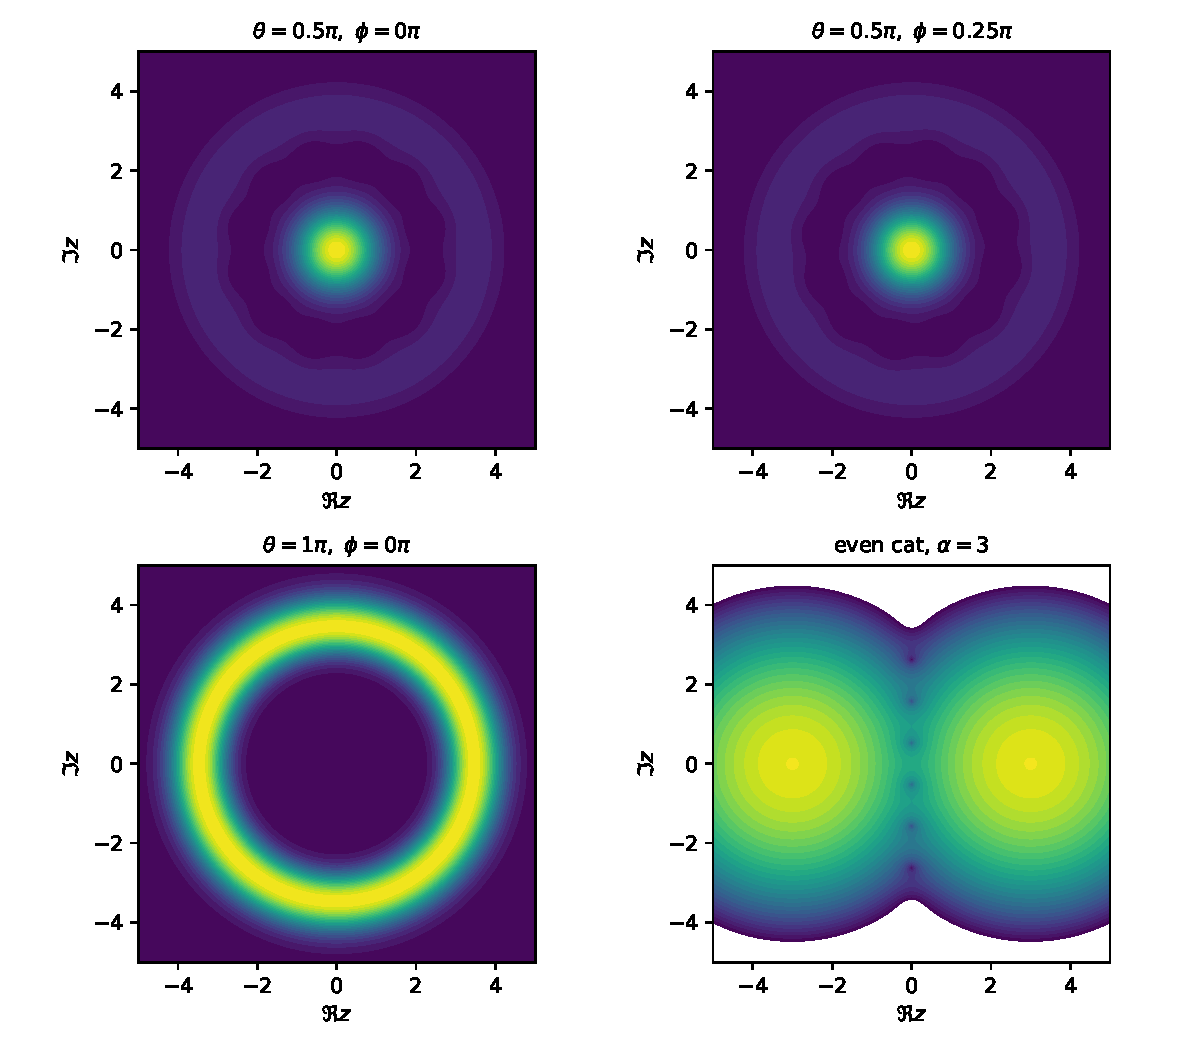
\includegraphics[width=\linewidth]{figures/quantum-states-1.pdf}\par
本图前三幅为8.422 HW1 P3(i), 第四为P3(ii)的偶猫对数Q. 改变相位旋转12折干涉瓣, 不改变两正交分量的二阶方差. 偶猫中心干涉来自相干振幅交叉项.

\originalsection{相位局域化与压缩}
\noindent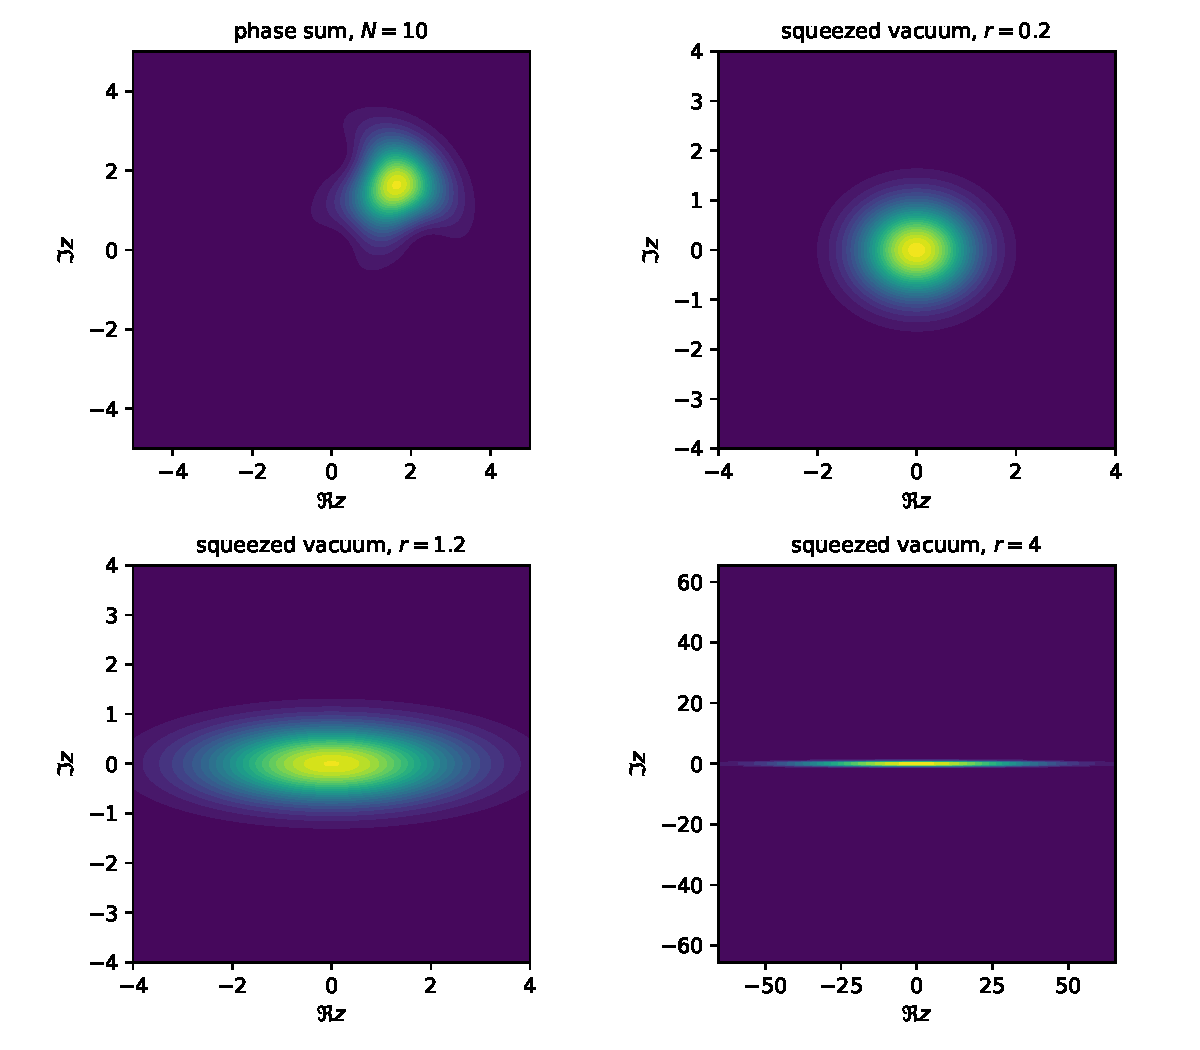
\includegraphics[width=\linewidth]{figures/quantum-states-2.pdf}\par
首幅为N=10相位和, 其二阶矩的最小正交方差约0.610, 未低于真空1/4. 后三幅是不同压缩参数的Q; Q把真实正交分量分布与测量真空噪声卷积, 因而窄轴不会像真实压缩方差那样无限趋零.

\originalsection{Kerr演化}
\noindent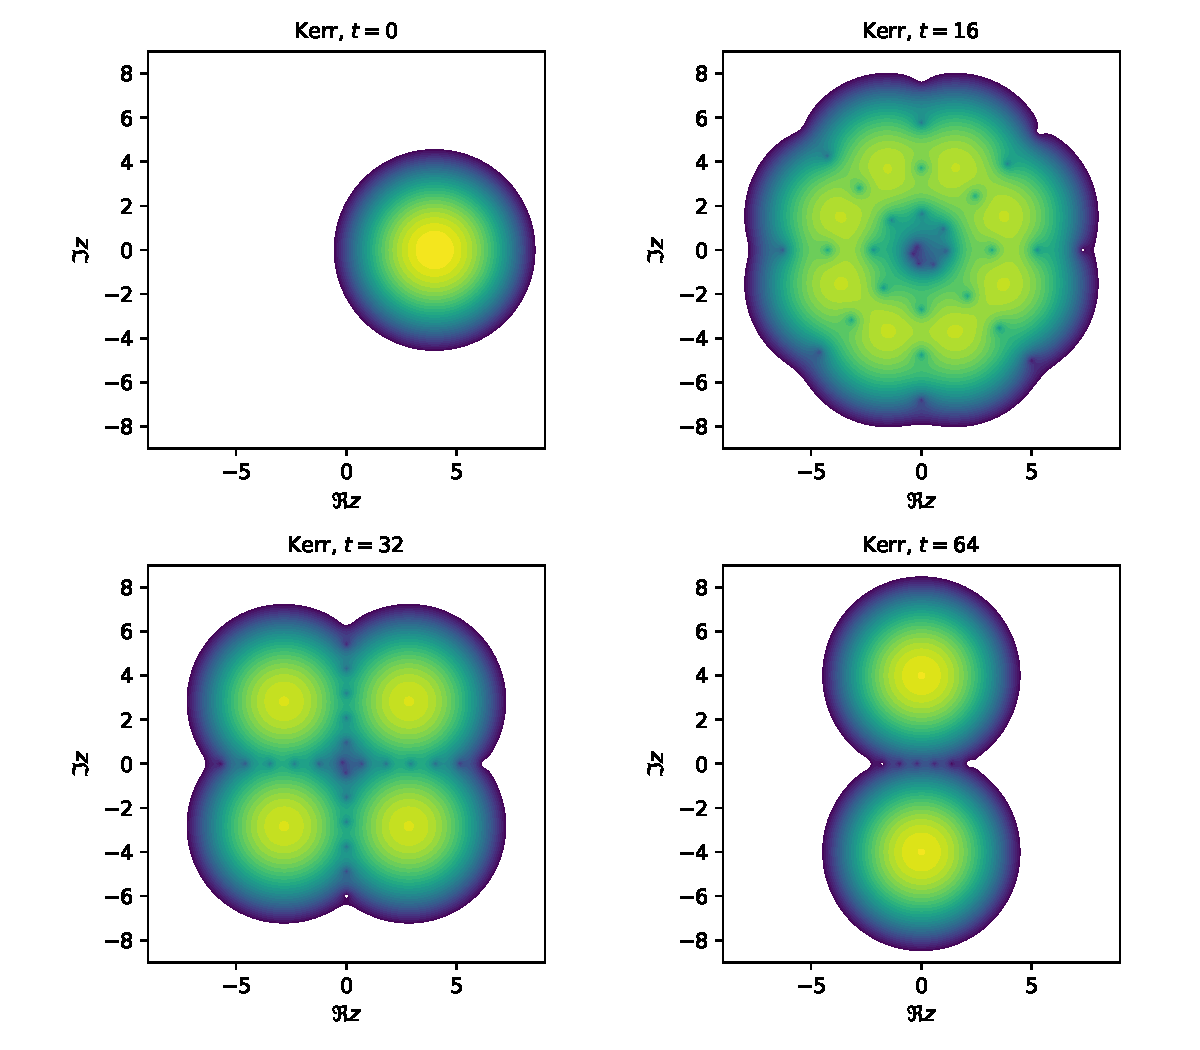
\includegraphics[width=\linewidth]{figures/quantum-states-3.pdf}\par
$t=64$时形成旋转后的双相干猫, $t=128$复现初态. 这组图对应$\xi=\pi/128$, 时间为题给无量纲单位, 不能直接读作秒.\par
\noindent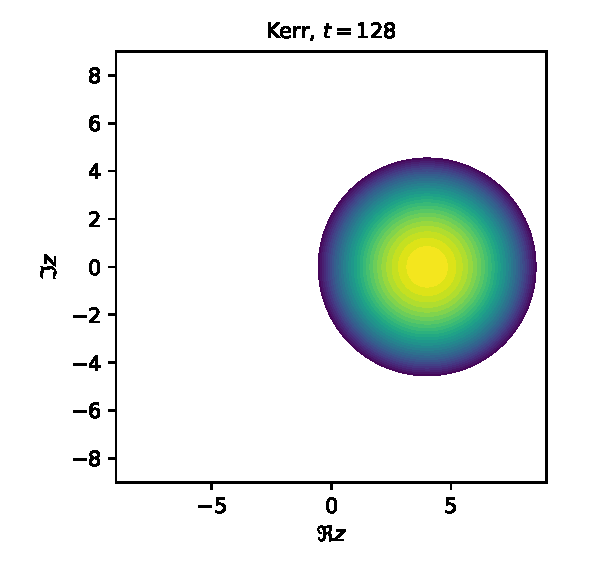
\includegraphics[width=.46\linewidth]{figures/quantum-states-4.pdf}\par
复现图与$t=0$相同至数态截断误差.

\originalsection{Schmidt阈值}
\noindent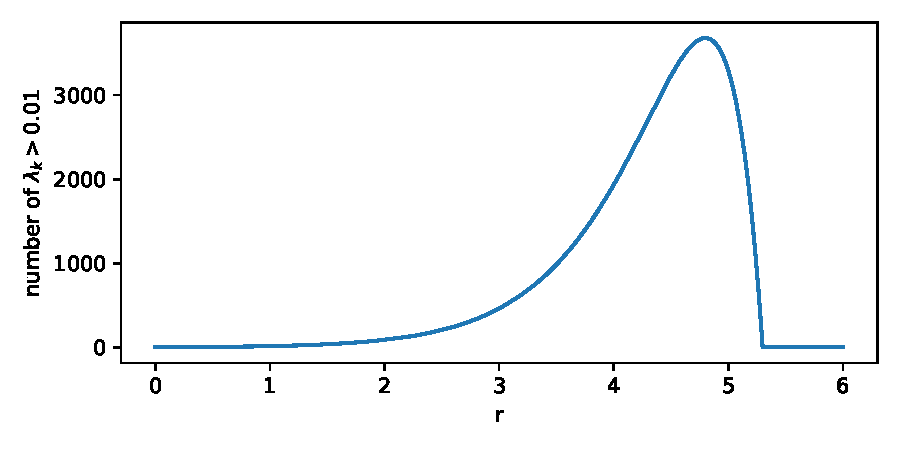
\includegraphics[width=.8\linewidth]{figures/schmidt-threshold.pdf}\par
固定系数阈值0.01的计数先增加后下降, $r\ge5.298$为零, 与真实纠缠熵的单调增长不同. 这实际反驳8.422 HW2 P3(e)的全区间单调目标.

\Needspace{12\baselineskip}
\originalsection{题目要求的能级与关联示意}
\begin{center}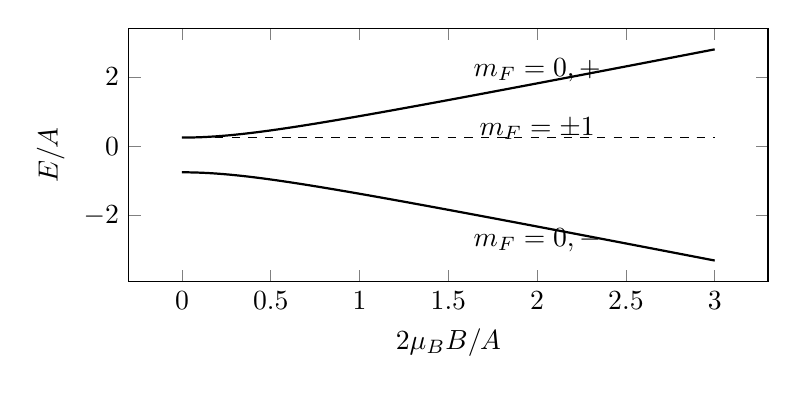
\begin{tikzpicture}\begin{axis}[width=.8\linewidth,height=4.8cm,xlabel={$2\mu_BB/A$},ylabel={$E/A$},domain=0:3,samples=80]
\addplot[thick]{-.25+sqrt(.25+x*x)};\addplot[thick]{-.25-sqrt(.25+x*x)};\addplot[dashed]{.25};
\node at(axis cs:2,.5){$m_F=\pm1$};\node at(axis cs:2,2.2){$m_F=0,+$};\node at(axis cs:2,-2.7){$m_F=0,-$};
\end{axis}\end{tikzpicture}\end{center}
2008期中第1题的正电子素图, 核与电子磁矩反号同大. 虚线表示两条重合水平能级, 不是只存在一个态.

\begin{center}\begin{tikzpicture}\begin{axis}[width=.8\linewidth,height=4.5cm,xlabel={$r_l\gamma/2$},ylabel={归一二粒子关联},domain=-3:3,samples=120,ymin=0,ymax=2.2]
\addplot[thick]{1+exp(-x*x)};\addplot[dashed,thick]{1-exp(-x*x)};\node at(axis cs:1,1.8){玻色};\node at(axis cs:1,.3){费米};
\end{axis}\end{tikzpicture}\end{center}
8.422 HW4 P2的Gaussian纵向平均关联. 曲线在零距离表现聚束和反聚束, 远处分布归一到1.

\begin{center}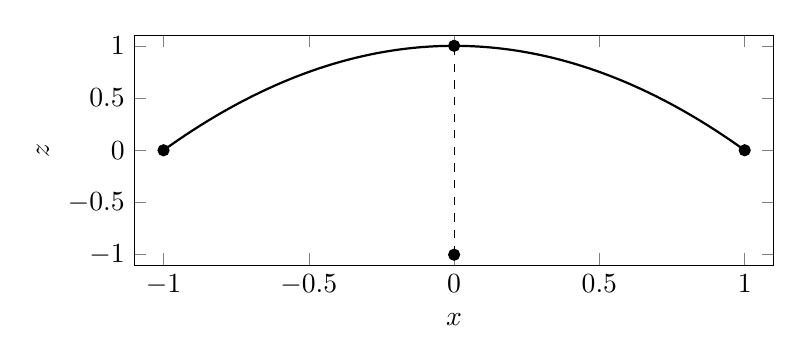
\begin{tikzpicture}\begin{axis}[width=.8\linewidth,height=4.5cm,xlabel={$x$},ylabel={$z$},xmin=-1.1,xmax=1.1,ymin=-1.1,ymax=1.1]
\addplot[domain=-1:1,samples=80,thick]{1-x*x};\addplot[domain=-1:1,samples=2,dashed]coordinates{(0,-1)(0,1)};
\addplot[only marks]coordinates{(-1,0)(1,0)(0,-1)(0,1)};
\end{axis}\end{tikzpicture}\end{center}
8.422 HW7 P2(e)的Bloch截面, 两等幅叠加沿抛物线趋向北极$g$, 纯激发态沿轴趋向同一点; 此图去掉了可逆自由进动.

\begin{center}\begin{tikzpicture}[>=Stealth]
\draw[->](-1,0)--(4,0)node[right]{$X$};\draw[->](0,-1.3)--(0,1.3)node[above]{$Y$};
\draw[dashed](0,0)ellipse(.35 and 1);\draw[thick,structurecolor](2,0)ellipse(.4 and 1.05);
\draw[->](.5,.7)--(1.8,.7)node[midway,above]{位移};
\end{tikzpicture}\end{center}
8.422 HW3 P3(c)沿低噪声X轴的相干位移. 输出椭圆比无损输入略扩大是混入端口噪声, 图仅示意方向与位置, 精确方差由该题公式给出.
